\documentclass[a4paper, 11pt]{article}

%%%%%% use packages %%%%%%
\usepackage{CJKutf8}
\usepackage{graphicx}
\usepackage[unicode]{hyperref}
\usepackage{indentfirst}
\usepackage{latexsym}
\usepackage{amsmath}
\usepackage{flafter}
\usepackage{enumerate}
\usepackage{leftidx}

%%%%%% indent settings %%%%%%
\setlength{\parindent}{20pt}
\setlength{\parskip}{1ex plus 0.5ex minus 0.25ex}
\setlength{\baselineskip}{1.0ex}
\renewcommand{\baselinestretch}{1.5}

\begin{CJK}{UTF8}{gbsn}


\title{CS61第九次课程记录}
\author{傅海平\\
\textsc{Institute Of Computing Technology,}\\
\textsc{Chinese Academy Of Sciences}\\
haipingf@gmail.com\\
}
\date{\today}
\begin{document}
\maketitle
\newpage
\tableofcontents
\newpage
\section{Topics}
\begin{center}
  \Large{线程}
\end{center}

\section{progress}
晚上7:30点开始,7:30 - 10:00 学习 lec17-threads.pdf 课程讲义,然后10:00开始讨论学习过程中遇到的问题。
\section{learning details}
\subsection{course sketch}
\subsubsection{Threads: Allowing a single program to do
multiple things concurrently.}
\begin{itemize}
  \item{并行编程}
	\begin{itemize}
	  \item{许多程序都需要并行执行:}
	  \item{浏览器}
	  \item{服务器}
	  \item{科学计算}
	  \end{itemize}
	\item{利用进程可以达到程序的并行执行}
	\item{但是,进程不太高效}
	  \begin{itemize}
		\item{每个进程有自己的也表,文件表,sockets\dots}
		\item{所以进程切换时代价较大,1.7KB的 $task\_struct$.}
		\item{进程的创建代价大。}
		\end{itemize}
	  \item{进程并不直接共享内存}
		\begin{itemize}
		  \item{并行程序需要对相同的内存区域进行操作。}
		  \item{许多 OS 提供了进程间通信的手段,如共享内存,$shmget(),
			shmat()$}
		  \end{itemize}
		\item{更好的办法}
		  \begin{itemize}
			\item{任务间共享了什么?}
			  \begin{itemize}
				\item{相同的代码}
				\item{相同的数据}
				\item{优先级}
				\item{某些系统资源:文件,sockets\dots}
				\end{itemize}
			\item{每个任务间哪些东西是私有的?}
			  \begin{itemize}
				\item{执行状态:CPU 寄存器,栈,和程序计数器PC}
				\end{itemize}
			  \item{线程}
			\end{itemize}
		  \item{线程和进程}
			\begin{itemize}
			  \item{线程与进程的相同点和区别}
			  \item{每个线程有自己的栈,栈指针,PC,和一些 CPU 寄存器,但共享相同
				的地址空间和系统资源,由于线程共享内存,所以方便线程间通信}
			  \end{itemize}
\end{itemize}
\begin{figure}[htbp]
  \centering
  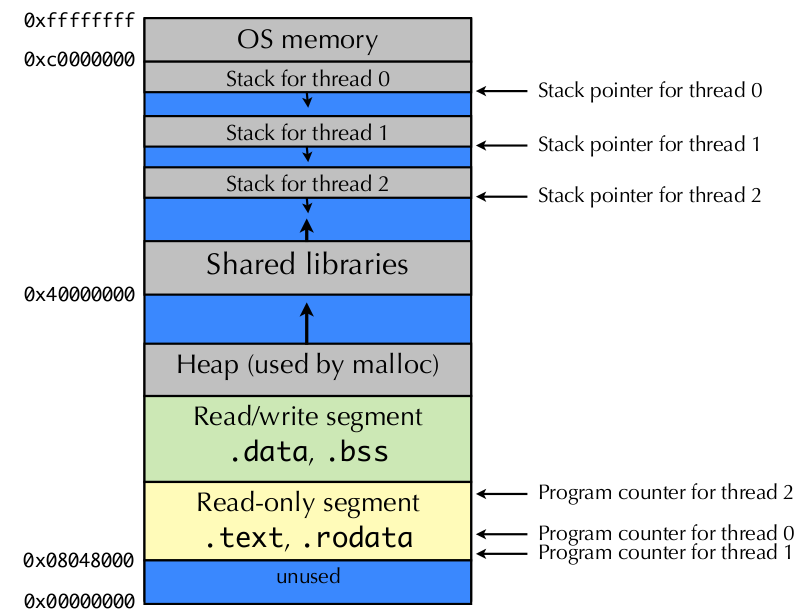
\includegraphics[width=10cm, keepaspectratio]{thread-va.png}
  \par\vspace{0pt}
  \rule{10cm}{0.1ex}
  \par{图1: 引入线程后,程序的进程空间}
\end{figure}
\subsubsection{Implementing}
\begin{itemize}
  \item{线程控制块TCB vs. 进程控制块PCB}
  \item{每个线程控制块内部都有指针指向相关的进程控制块。}
  \item{TCB包含了与线程相关的信息,处理器状态和指向PCB的指针}
  \item{PCB 包含了进程的相关信息,如地址空间,系统资源,但是没有处理器状态}
  \item{Linux:TCB(thread\_struct), PCB(task\_struct)}
  \item{用户空间的线程实现}
	\begin{itemize}
	  \item{setcontext, getcontext, makecontext, swapcontext}
	  \item{int setcontext(const ucontext\_t *ucp) }
		\begin{itemize}
		  \item{This function transfers control to the context in ucp. Execution
			continues from the point at which the context was stored in ucp.
			setcontext does not return.}
		  \end{itemize}
		
		\item{int getcontext(ucontext\_t *ucp) }
		\begin{itemize}
		  \item{Saves current context into ucp. This function returns in two
			possible cases: after the initial call, or when a thread switches to
			the context in ucp via setcontext or swapcontext. The getcontext
			function does not provide a return value to distinguish the cases
			(its return value is used solely to signal error), so the programmer
			must use an explicit flag variable, which must not be a register
			variable and must be declared volatile to avoid constant propagation
			or other compiler optimisations.}	
		  \end{itemize}

		\item{void makecontext(ucontext\_t *ucp, void *func(), int argc, \dots)}
		\begin{itemize}
		  \item{The makecontext function sets up an alternate thread of control
			in ucp, which has previously been initialised using getcontext. The
			ucp.uc\_stack member should be pointed to an appropriately sized
			stack; the constant SIGSTKSZ is commonly used. When ucp is jumped to
			using setcontext or swapcontext, execution will begin at the entry
			point to the function pointed to by func, with argc arguments as
			specified. When func terminates, control is returned to ucp.uc\_link.}
		  \end{itemize}

		\item{int swapcontext(ucontext\_t *oucp, ucontext\_t *ucp) }
		\begin{itemize}
		  \item{Transfers control to ucp and saves the current execution state
			into oucp. }
		  \end{itemize}

	  \end{itemize}
  \end{itemize}
\subsubsection{Scheduling}
\begin{itemize}
  \item{线程是CPU调度的基本单位。}
  \item{上下文切换}
  \item{抢占调度}
  \item{协同调度}
  \end{itemize}
\subsubsection{Programming with threads (pthreads library)}
\begin{itemize}
  \item{Pthread}
	\begin{itemize}
	  \item{线程的创建,终结}
	  \item{同步}
	  \item{通信}
	  \end{itemize}
  \item{Pth}
  \item{Pthread: API}
	\begin{itemize}
	  \item{pthread\_create}
	  \item{pthread\_self}
	  \item{pthread\_exit}
	  \item{pthread\_cancel}
	  \item{pthread\_join}
	  \end{itemize}
  \end{itemize}
\subsubsection{Shared vs. private resources}

\subsubsection{The need for synchronization}
\subsection{Problems}
\subsection{Solutions}
\end{CJK}
\end{document}
